% Copyright Aidan Randle-Conde 2007-2014
% http://www.aidansean.com/phd_notes
% Anyone is free to download, redistribute, edit and use these notes and the source tex files with the following restrictions:
% This 
%  This message is included in the tex source files.
%  Aidan Randle-Conde is credited as the author.
%  Images are correctly credited to their respective authors, as outlined in the references.
%  No part of these notes may be used for commercial purposes.

\chapter{Experiments of the past fifty years}

Until the 1950s particle physics was studied by observing cosmic rays in cloud chambers and nuclear emulsion.  After 1945 nucleon-nucleon scattering experiements were carried out at cyclotrons and energies became high enough for pions to be produced.  Then pion-nucleon scattering was studied.

\[
  \textrm{In 1952 } \pi^+ \quad p \stackrel{\Delta^{++}}{\to} \pi^+ \quad p
\]

Also, from electron beams photons could be produced:

\[
  \gamma \quad p \stackrel{\Delta^+}{\to} \gamma \quad \gamma \quad p \quad (\textrm{via } \Delta^+ \to p \quad \pi^0 )
\]

although the rate of production via $\gamma$ processes is much lower because of the strength of the electromagnetic coupling.

Other processes were also observed:
\begin{eqnarray*}
  \pi^+ & \to & \mu^+ \quad \nu_{\mu} \\
  \mu^+ & \to & \e^+ \quad \bar{\nu}_{\mu} \quad \nu_e
\end{eqnarray*}

where the latter process is a purely leptonic process and so provoked much theoretical interest.

In 1956 parity violation in the weak interaction was discovered (Lee and Young received the Nobel Prize.)  The experiement was studying the $\beta$ decay of polarised Cobalt $60$ nuclei.  An anistropy was discovered in the electron spectroscopy with respect to the $^{60}\textrm{Co}$ nuclear spin. The spins of the particles are shown in figure \ref{fig:ch3_CoNi}.

\begin{figure}
  \begin{center}
    \begin{tabular}{ccccccc}
      $\textrm{Co}$      &               & $\textrm{Ni}$      &     &            &               &                   \\
                         &               &                    &     & $\Uparrow$ & $\bar{\nu}_e$ & $\uparrow$        \\
      $\Big{\Uparrow}$   & $\rightarrow$ & $\Big{\Uparrow}$   & $+$ &            &               &                   \\
                         &               &                    &     & $\Uparrow$ & $e^-$         & $\downarrow$      \\
      $J=5$              &               & $J=4$              &     &            &               &                   \\
      &&&&&&\\
      $^{60}\textrm{Co}$ & $\rightarrow$ & $^{60}\textrm{Ni}$ & $+$ & $(e^-)_L$  & $+$           & $(\bar{\nu}_e)_R$ \\
    \end{tabular}
  \caption{Parity violating decay $^{60}\textrm{Co}\to ^{60}\textrm{Ni}\, e^- \,\bar{\nu}_e$}
  \label{fig:ch3_CoNi}
  \end{center}
\end{figure}

\[
  ^{60}\textrm{Co} \to ^{60}\textrm{Ni}* \Big(\e^-\Big)_L \Big(\bar{\nu}_e\Big)_R
\]

By the 1960s kaon beams were generated at synchotrons and this confirmed the discovery of strangeness that was observed in cosmic ray experiments.  It also established (in the experimentalists' eyes) the quark substructure of hadrons ie hadrons were made of $q\bar{q}$ pairs (mesons) and $qqq$ triplets (baryons) where $q$ is a $u$, $d$ or $s$ quark.  Theorists regarded the evidence for strangeness as establishing the $SU(3)$ flavour symmetry, which is now known to have been accidental.  This symmetry arises because the constituent masses of $u$ and $d$ quarks are about the same and the mass of the $s$ quark is somewhat heavier.

\section{Mesons and baryons}

Consider $q\bar{q}$ systems consisting of $u$ and $d$ quarks.  The strong isospin doublet is:

\[
  2 = 
  \left(
    \begin{array}{c}
    u \\
    d
    \end{array}
  \right)
    \begin{array}{ccc}
    I_3 & = & \pm \frac{1}{2} \\
    I & = & \frac{1}{2}
    \end{array}
\]

Assume that the strong isospin is conserved (which is accidental, but works as the $u$ and $d$ quarks have nearly the same mass.)  This doublet is combined with the antiquark doublet which is:

\[
  \bar{2} = 
  \left(
    \begin{array}{c}
    -\bar{d} \\
    \bar{u}
    \end{array}
  \right)
    \begin{array}{c}
    ^{ \frac{1}{2}} \\
    _{-\frac{1}{2}}
    \end{array}
\]

In this form the raising and lowering operators act on the $2$ doublet in the same way for the $\bar{2}$ antiquark doublet.  The minus sign on $\bar{d}$ arises because of a rotation in isospin space:

\begin{eqnarray*}
  \left(
    \begin{array}{c}
    u \\
    d
    \end{array}
  \right)'
  & = &
  \e^{-i \pi \tau_z/2}
  \left(
    \begin{array}{c}
    u \\
    d
    \end{array}
  \right)
  \\
  & = &
  I\left( \cos \frac{\pi}{2} -i\frac{\tau}{2} \sin \frac{\pi}{2} \right)
  \left(
    \begin{array}{c}
    u \\
    d
    \end{array}
  \right)
  \\
  \Rightarrow
  \left(
    \begin{array}{c}
    u \\
    d
    \end{array}
  \right)'
  & = &
  \left(
    \begin{array}{cc}
    0 & -1 \\
    1 & 0
    \end{array}
  \right)
  \left(
    \begin{array}{c}
    u \\
    d
    \end{array}
  \right)
  \\
  & = &
  \left(
    \begin{array}{c}
    -d \\
    u
    \end{array}
  \right)
  \\
  u' & \to & -d \\
  d' & \to & u
\end{eqnarray*}

Suppose $\bar{2}$ had been defined as:

\[
  \bar{2} = 
  \left(
    \begin{array}{c}
    \bar{d} \\
    \bar{u}
    \end{array}
   \right)
\]

Then the transformation would be:

\begin{eqnarray*}
  \bar{d}' & \to & -\bar{u} \\
  \bar{u}' & \to & \bar{d}
\end{eqnarray*}

The $\bar{2}$ system therefore transforms in the same way as a the $2$ system:

\begin{eqnarray*}
  \left(
    \begin{array}{c}
    -\bar{d} \\
    \bar{u}
    \end{array}
  \right)
  & = &
  \left(
    \begin{array}{cc}
    0 & -1 \\
    1 & 0
    \end{array}
  \right)
  \left(
    \begin{array}{c}
    -\bar{d} \\
    \bar{u}
    \end{array}
  \right)
  \\
  & = &
  \left(
    \begin{array}{c}
    -\bar{u} \\
    -\bar{d}
    \end{array}
  \right) \\
  -\bar{d}' & \to & -\bar{u} \\
  \bar{u}'  & \to & -\bar{d}
\end{eqnarray*}

Now $2$ and $\bar{2}$ can be combined to form a representation of the $\pi$ mesons:

\[
  \begin{array}{ccccc}
           & ( & u         & d         & ) \\
  \left( \begin{array}{c}-\bar{d} \\ \bar{u} \end{array} \right) & \Bigg( 
  & \begin{array}{c} -u\bar{d} \\ u\bar{u} \end{array}
  & \begin{array}{c} -d\bar{d} \\ d\bar{u} \end{array} & \Bigg) \\
  \end{array}
\]

\begin{eqnarray*}
  \pi^+ & = & -u\bar{d} \\
  \pi^- & = & d\bar{u} \\
  \pi^0 & = & \frac{1}{\sqrt{2}}\left( u\bar{u} - d\bar{d} \right)
\end{eqnarray*}

There is an isospin doublet to represent the antiquarks in $SU(2)$ and not in any other $SU(n)$.  In $SU(3)$ flavour symmetry:

\begin{eqnarray*}
  3 & = &
  \left(
    \begin{array}{c}
    u \\
    d \\
    s
    \end{array}
  \right)
  \\
  \bar{3} & = &
  \left(
    \begin{array}{c}
    \bar{u} \\
    \bar{d} \\
    \bar{s}
    \end{array}
  \right)
\end{eqnarray*}

To construct the $q\bar{q}$ states in $SU(3)$:

\[
  \begin{array}{cccccc}
    & ( & u & d & s & ) \\
    \left(
    \begin{array}{c}
      \bar{u} \\
      \bar{d} \\
      \bar{s}
    \end{array}
    \right)
    &
    \Bigg(
    &
    \begin{array}{c}
      u\bar{u} \\
      u\bar{d} \\
      u\bar{s}
    \end{array}
    &
    \begin{array}{c}
      d\bar{u} \\
      d\bar{d} \\
      d\bar{s}
    \end{array}
    &
    \begin{array}{c}
      s\bar{u} \\
      s\bar{d} \\
      s\bar{s}
    \end{array}
    &
    \Bigg)
  \end{array}
\]

The non diagonal elements are easily identified as the following particles:

\begin{eqnarray*}
  s\bar{u} = K^- & & u\bar{s} = K^+ \\
  d\bar{s} = \bar{K}^0 & & s\bar{d} = K^0 \\
  u\bar{d} = \pi^+ & & d\bar{u} = \pi^-
\end{eqnarray*}

There is also a symmetric state:

\[
  \eta_1: \quad \frac{1}{\sqrt{3}}\left( u\bar{u} + d\bar{d} + s\bar{s} \right)
\]

This is called the $SU(3)$ singlet state.  The final neutral state is:

\[
  \eta_8: \quad \frac{1}{\sqrt{6}}\left(u\bar{u} + d\bar{d} + 2s\bar{s} \right)
\]

This is constructed to be orthogonal to the $\pi^0$ and the singlet state.  The mesons are shown in figures \ref{fig:ch3_mesonNonetSpin0} and \ref{fig:ch3_mesonNonetSpin1}.

\begin{figure}[!htb]
  \begin{center}
    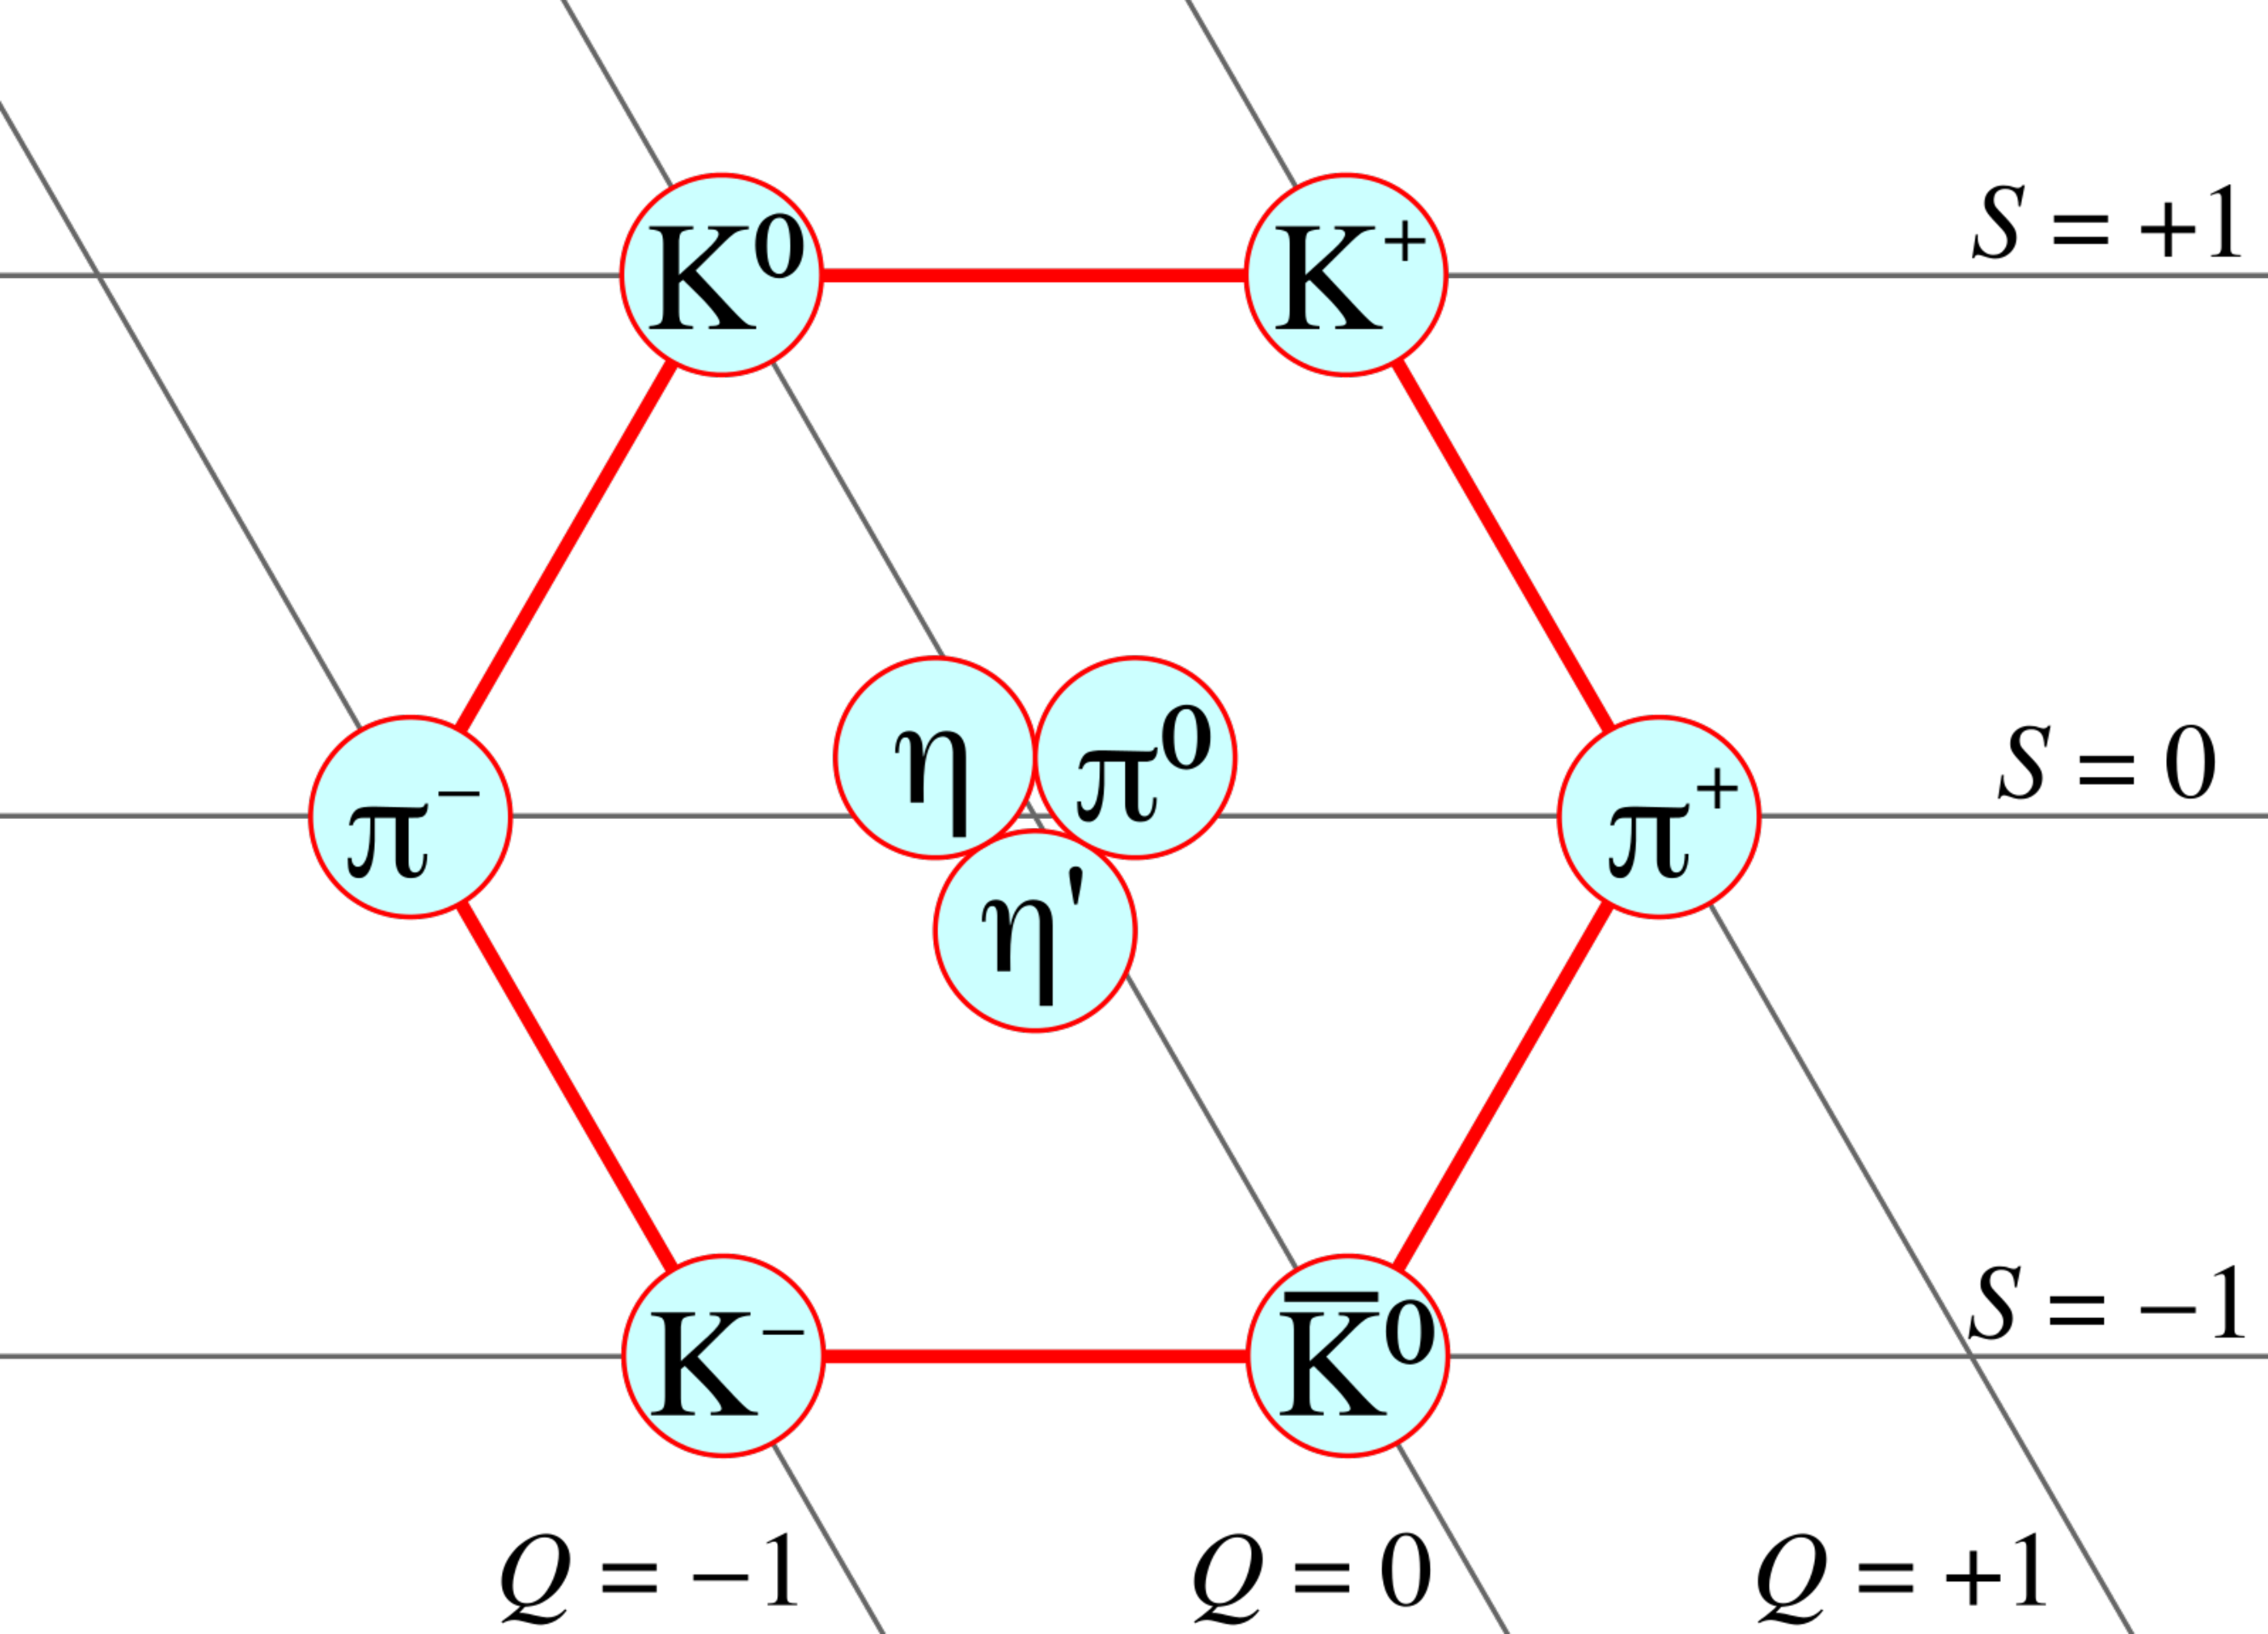
\includegraphics[width=0.5\textwidth]{images/chapter_3/MesonNonetSpin0.pdf}
    \caption[$J^{P}=0^-$ meson nonet]{The pseudoscalar $J^{P}=0^-$ meson nonet. \cite{mesonNonets}}
    \label{fig:ch3_mesonNonetSpin0}
  \end{center}
\end{figure}

\begin{figure}[!htb]
  \begin{center}
    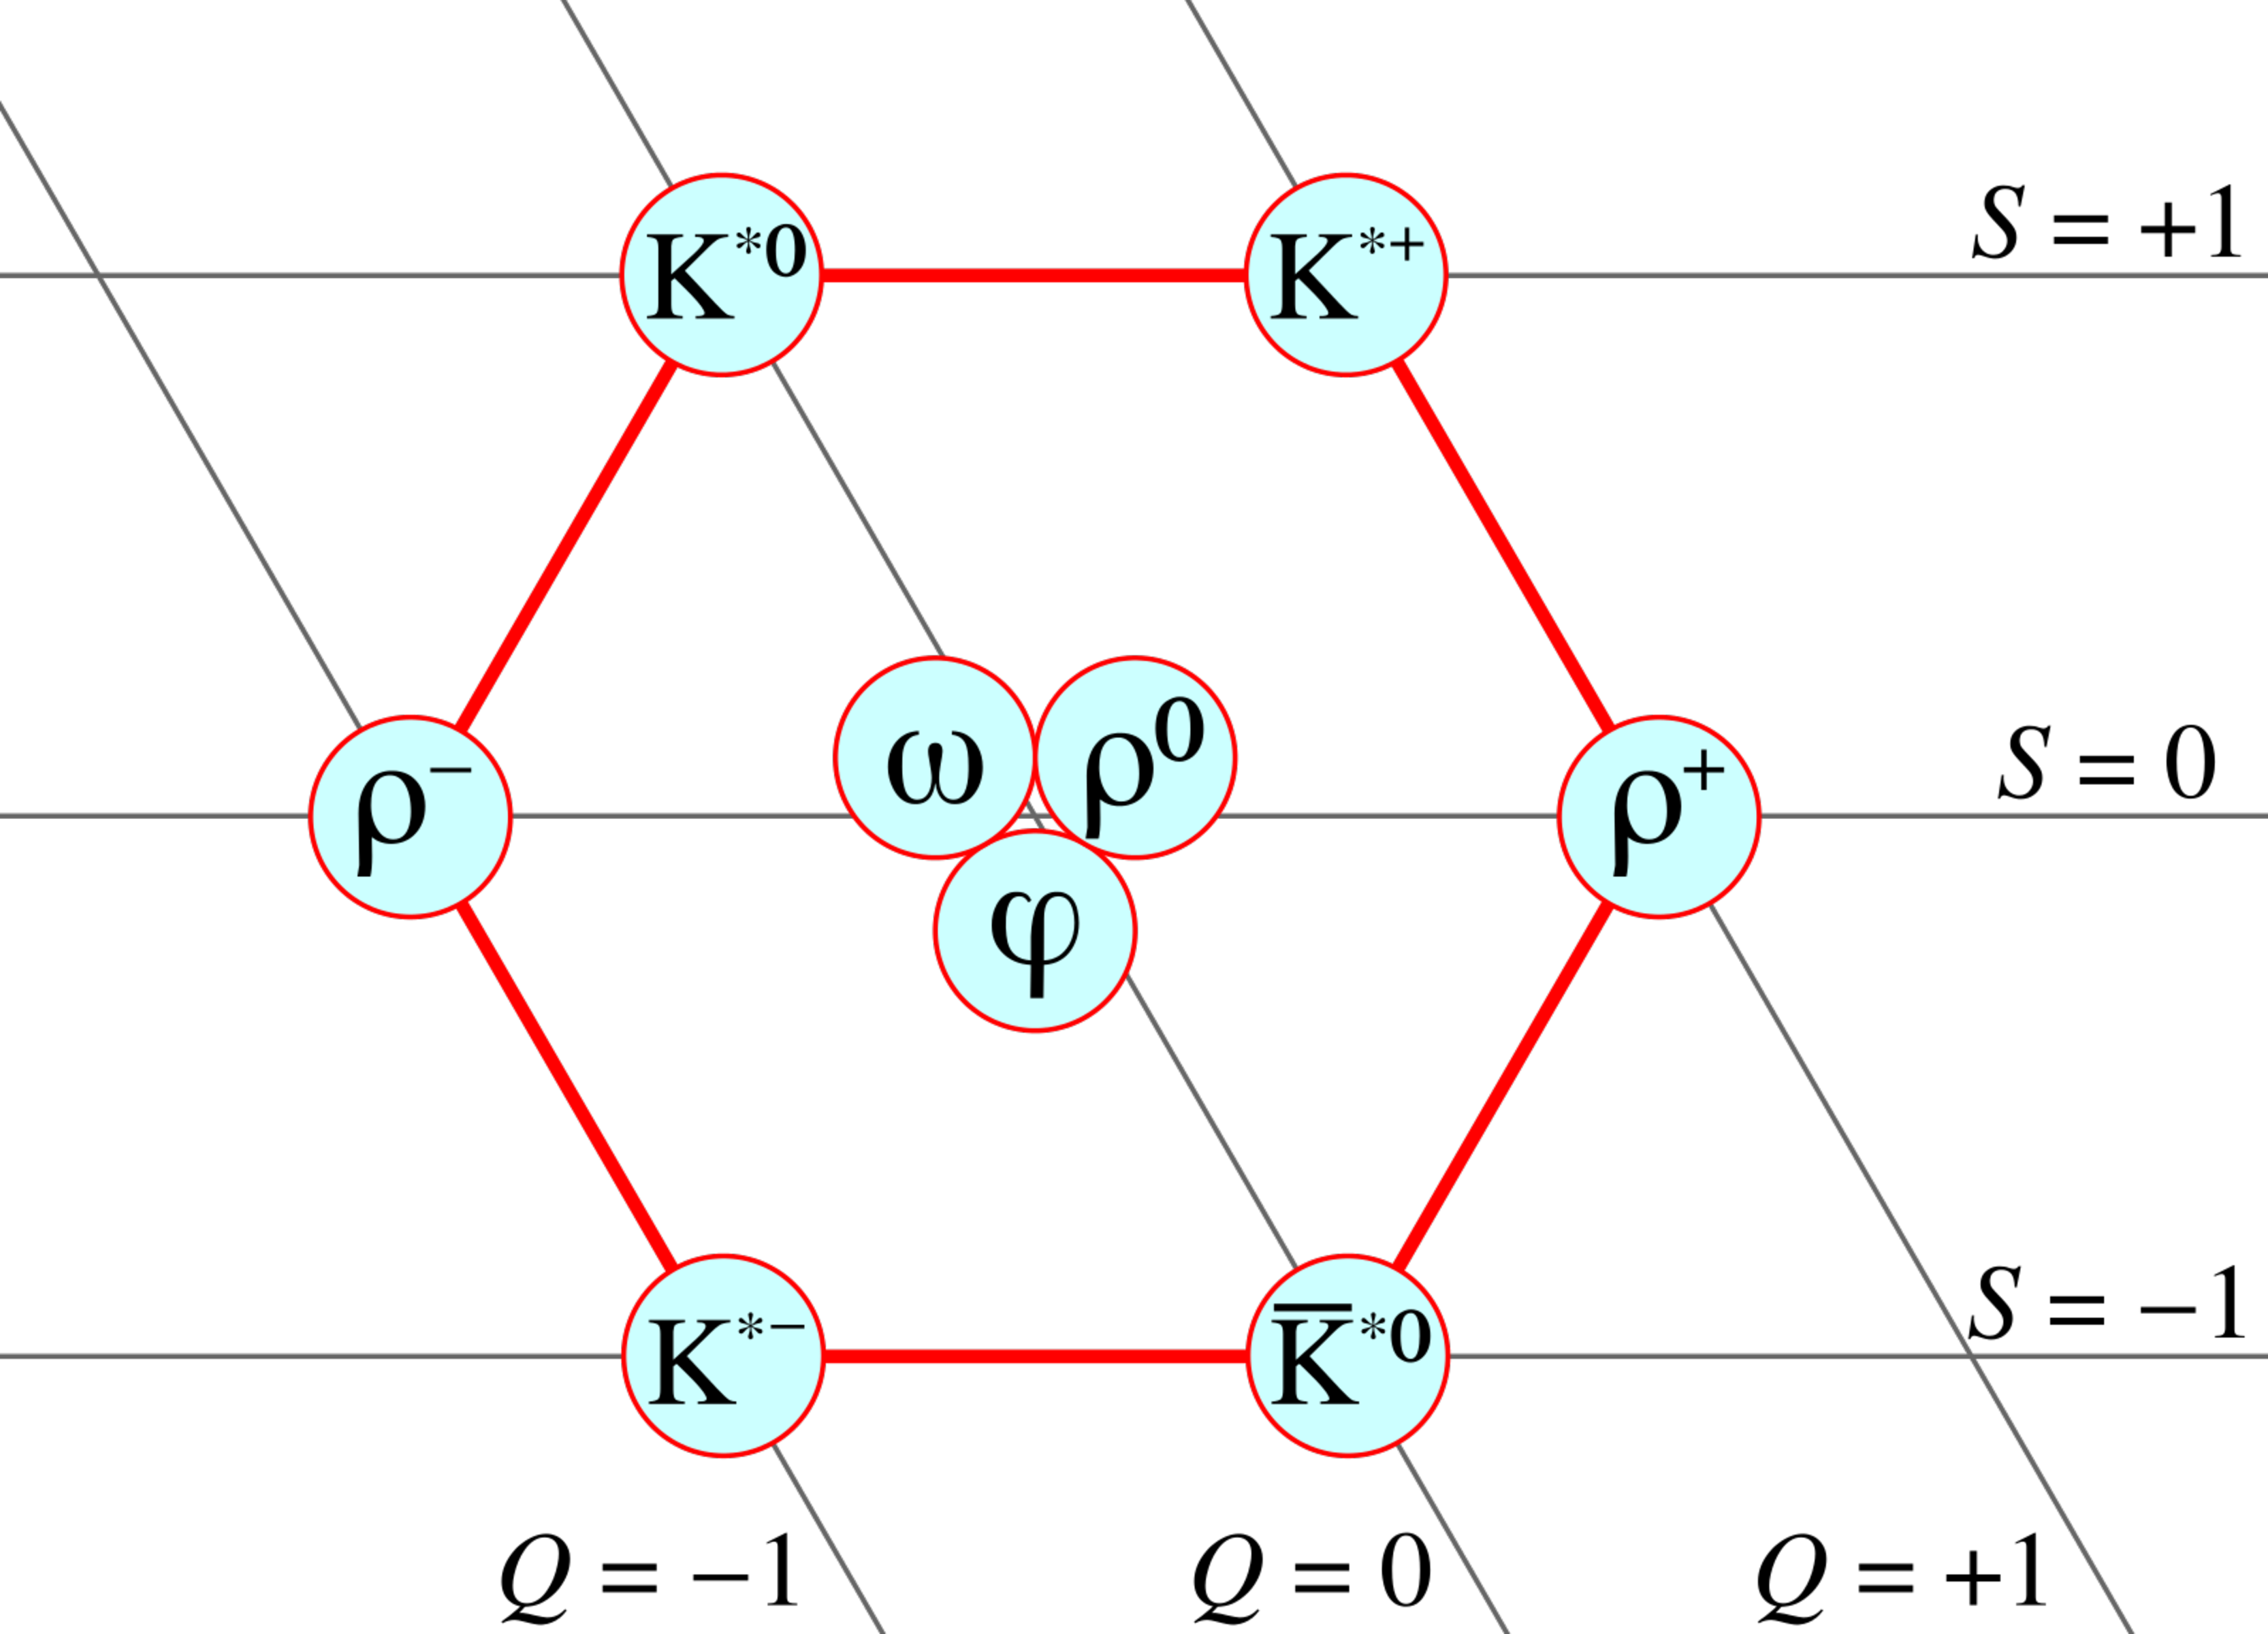
\includegraphics[width=0.5\textwidth]{images/chapter_3/MesonNonetSpin1.pdf}
    \caption[$J^{P}=1^-$ meson nonet]{The vector $J^{P}=1^-$ meson nonet. \cite{mesonNonets}}
    \label{fig:ch3_mesonNonetSpin1}
  \end{center}
\end{figure}

\clearpage

\section{Neutrino experiments}

\subsection{The Gargamelle experiment}

Using the CERN proton synchrotron, protons were extracted from the accelerator and impinged on a thin Beryllium target within a neutrino horn.  In the targets $\pi$s and $K$s were created and the horn partially selected either positive or negative charges.  The partially focussed $\pi^+$ beam decayed to $\mu^+ \nu_{\mu}$.  An iron shield filtered out the remaining hadrons and muons.  Measurements of the muon tracks enabled the neutrino spectrum to be determined.  The neutrios then passed into the large heavy liquid bubble chamber, Gargamelle.  Scattering via the exchange of the $W^{\pm}$ was expected, but scattering via the $Z^0$ was also observed, as shown in figure \ref{fig:ch3_NumPToMuHad}.

\begin{figure}[!htb]
  \begin{center}
    \begin{tabular}{cc}
      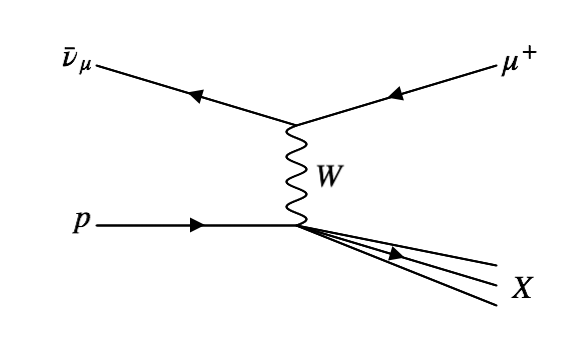
\includegraphics[width=0.45\textwidth]{images/web_feynman/image_9.png} &
      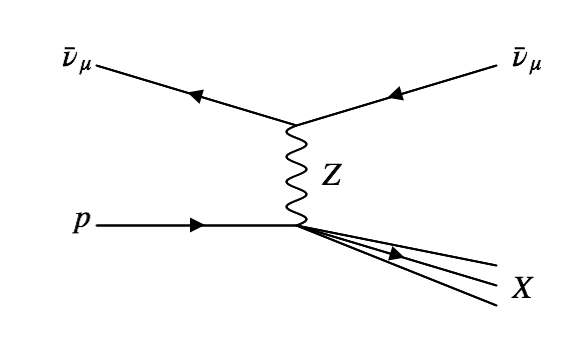
\includegraphics[width=0.45\textwidth]{images/web_feynman/image_10.png}
    \end{tabular}
    \caption[Neutrino-nucleon scattering at Gargamelle]{Neutrino-nucleon scattering at Gargamelle, with a charged current interaction (left), and neutral current interaction (right).}
    \label{fig:ch3_NumPToMuHad}
  \end{center}
\end{figure}

\subsection{Underground experiments}

Solar neutrinos are produced primarily by the following reaction:

\[
  p \quad p \to d \quad \e^+ \quad \nu_e
\]

Atmospheric neutrinos are produced primarily by proton bombardment of the upper atmosphere:

\[
  \begin{array}{ccccc}
  p \quad N & \to & \pi^+/K^+ \quad \textrm{H}      &                 & \\
      &     &  \hookrightarrow & \mu^+ \quad \nu_{\mu} & \\
      &     &                  & \hookrightarrow & \e^+ \quad \bar{\nu}_{\mu} \quad \nu_e
  \end{array}
\]

Naïvely, it is expected that the production rate would be:

\[
  \frac{\nu_e}{\nu_{\mu}} \sim \frac{1}{2}
\]

The ratio has been measured by Superkamikande to be closer to $1$, demonstrating that $\nu_{\mu}$ neutrinos were missing and also measured an azimuthal variation.  ie the experiment measured the number of neutrinos $N(\nu_{\mu})$ and $N(\nu_e)$ from the atmosphere (above) and the other side of the Earth (below.)  About half from the other side of the Earth were lost, suggesting that that neutrinos oscillated into $\nu_{\tau}$.  The oscillations imply that neurinos have mass and as such must have a velocity $\beta < 1$.

A large detector of water was used to look for the processes:

\begin{eqnarray*}
  \nu_{\mu} \quad N & \to & \mu^- \quad \textrm{H} \\
  \nu_e     \quad N & \to & \e^-  \quad \textrm{H}
\end{eqnarray*}

Both muons and electrons were detected by $\sim 5,000$ phototubes by considering their characteristic signals for Cerenkov light.  The muon signal rings are sharp whereas those for electrons are diffuse.

\subsection{Solar neutrinos}

In the experiment by Ray Davis mainly ``high'' energy ($14 \mev$) neutrinos were used from a process:

\[
  \begin{array}{cccc}
  p \quad ^7\textrm{Be} & \to & ^8\textrm{Be} \quad \gamma & \\
               &     & \hookrightarrow   & ^8\textrm{Be} \quad \e^+ \quad \nu_e
  \end{array}
\]

The group looked for the reaction:

\[
  \nu_e \, {}^{37}\textrm{Cl} \to \e^- \quad \phantom{}^{37}\textrm{Ar}
\]

The neutrinos were impinging on a tank of $C_2Cl_4$.  There were not as many such reactions as expected according to the Standard Model.

To detect low energy neutrinos, tanks of Galium were used:

\[
  \nu_e \quad \textrm{Ga} \to \textrm{Ge} \quad \e^-
\]

These processes were also observed at a lower than expected rate.

In the Sudbury Neutrino Observatory (SNO) a tank of heavy water ($\textrm{D}_2\textrm{O}$) was used.  The following reaction was detected:

\[
  \nu_e \quad n \to \e^- \quad p
\]

Again, a deficit of electron neutrinos was observed.  Around $1/3$ of the expected signal was observed.  Combined with the results from Superkamiokande this explains the solar neutrino problem where $\sim 1/3 \nu_e$ are observed and $\sim 2/3 \nu_e$ oscillate into $\nu_{\mu}$ and $\nu_{\tau}$.

The results at SNO were further confirmed when salt ($\textrm{NaCl}$) was added to the water, increasing the sensitivity to $\nu_{\mu}$ and $\nu_{\tau}$:

\begin{eqnarray*}
  \nu_{e/\mu/\tau} \quad n       & \to & \nu_{e/\mu/\tau} \quad n_{scattered} \\
  \textrm{Then } ^{37}\textrm{Cl} \quad n & \to & ^{38}\textrm{Be} \quad \gamma
\end{eqnarray*}

This was then consistent with the expected solar flux.

Further neutrino oscillation experiments are ongoing at reactors (a good source of copious low energy neutrinos from $b$ decay) and at accelerators such as MINOS.

\section{Colliding beam experiments (Some fixed target)}

There are various different types of colliding beams which have different properties and can probe different phenomena.  They can be classified into three types:

\begin{description}
  \item[$\e^+ \e^-$] Purely leptonic beams give rise to "clean" output and also have a controled centre of mass energy.  There is a large discovery potential, however there are limits due to synchrotron  radiation, so future developments will lead to linear colliders.
  \item[$NN(pp)$]   Purely hardonic beams are not as clean and do not have a well defined centre of mass energy.  However there is a large discovery potential due to the possibility of much higher energies.
  \item[$lN$]      A mixed pair of beams allows probing of the partons.
\end{description}

\subsection{Lepton-nucleon colliders}

In the late 1960s and the early 1970s deep inelastic scattering experiments using lepton beams of electrons, neutrinos and also muons were used to probe the structure of the proton and neutron.  It looked as if scattering occured on pointlike objects in the nucleon and around 50\% of the nucleon interacted in this way.  The remaining 50\% was made up of gluons.  This was the beginnings of quantum chromodynamics (QCD).

At HERA, this has been advanced further in $ep$ collisions.  Electrons (or positrons) of energies at $27.5 \gev$ collide with protons at $920 \gev$, yielding a centre of mass energy of around $320 \gev$.  There are two multipurpose colliding beam experiments which measure a wide range of phenomena such as proton and photon structure; many other aspects of QCD; electroweak physics and searches for effects beyond the Standard Model (eg leptoquarks).

The structure of the proton has been measured over a vast kinematic range compared to the first measurements in the 1960s, as shown in figure \ref{fig:ch3_F2}.  A typical deep inelastic scattering process is shown in figure \ref{fig:ch3_EPToEHad}.

\begin{figure}[!htb]
  \begin{center}
    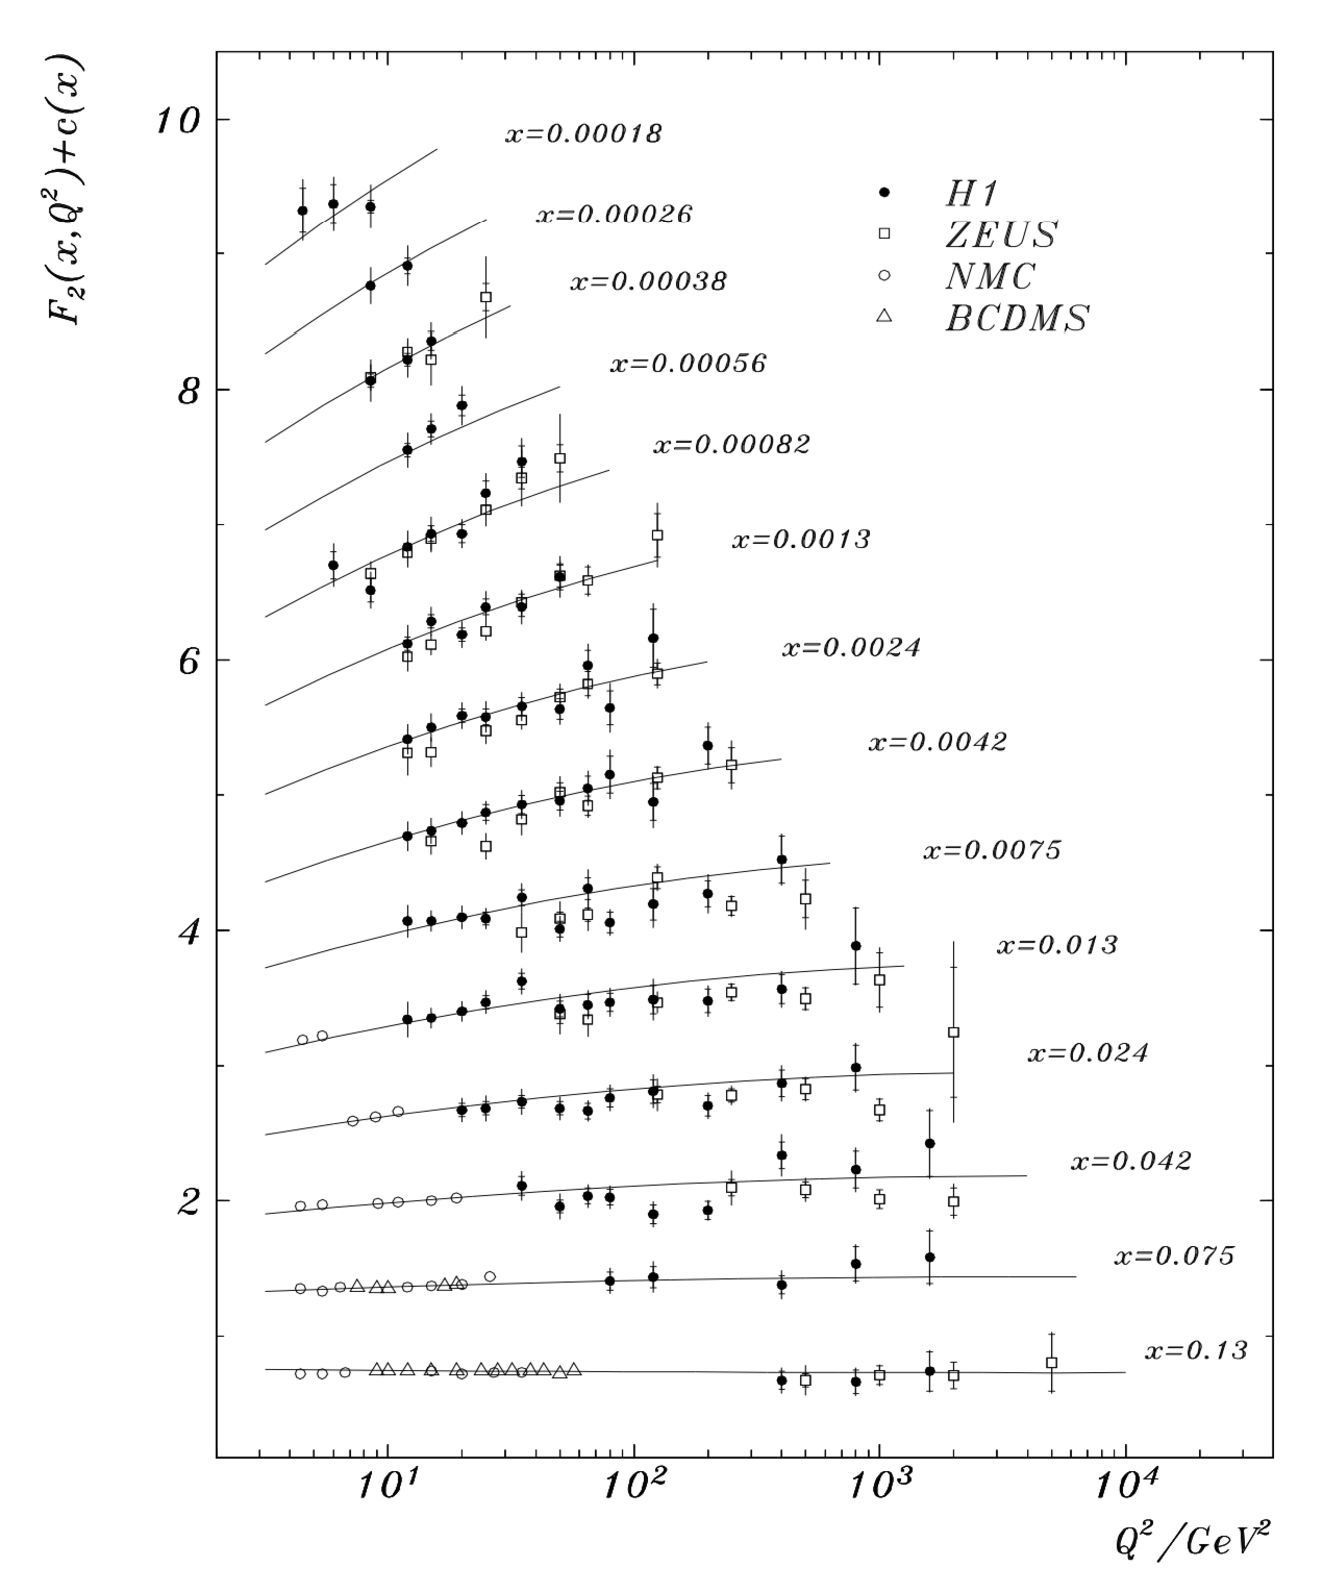
\includegraphics[width=0.7\textwidth]{images/chapter_3/F2.pdf}
    \caption[The structure of the proton]{The structure of the proton, $F_2$, as a function of $Q^2$. \cite{F2}}
    \label{fig:ch3_F2}
  \end{center}
\end{figure}

\begin{figure}[!htb]
  \begin{center}
    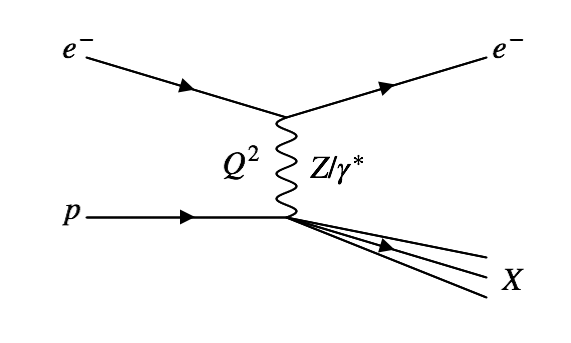
\includegraphics[width=0.8\textwidth]{images/web_feynman/image_11.png}
    \caption[Deep inelastic scattering process]{Deep inelastic scattering process for $e^-p\to e^-X$, where $X$ is any hadronic system allowed by conservation laws.}
    \label{fig:ch3_EPToEHad}
  \end{center}
\end{figure}

$x$ is the proton's momentum fraction carried by the struck quark.
$Q^2$ is the four momentum transfer, essentially related to the wavelength of the probing photon.  A high value for $Q^2$ implies a high resolving power.

This gives us precise knowledge of the structure of matter which is one of the fundamental goals of physics.  Also practically many colliders use protons (eg LHC) so it is useful for understand the structure of what is being collided.

Demonstration of the unification of the electroweak force is shown in figure \ref{fig:ch3_electroweakUnification}.  The processes became the ``same'' at $M^2_{W,Z} \sim 10^4 \gev^2$.

\begin{figure}[!htb]
  \begin{center}
    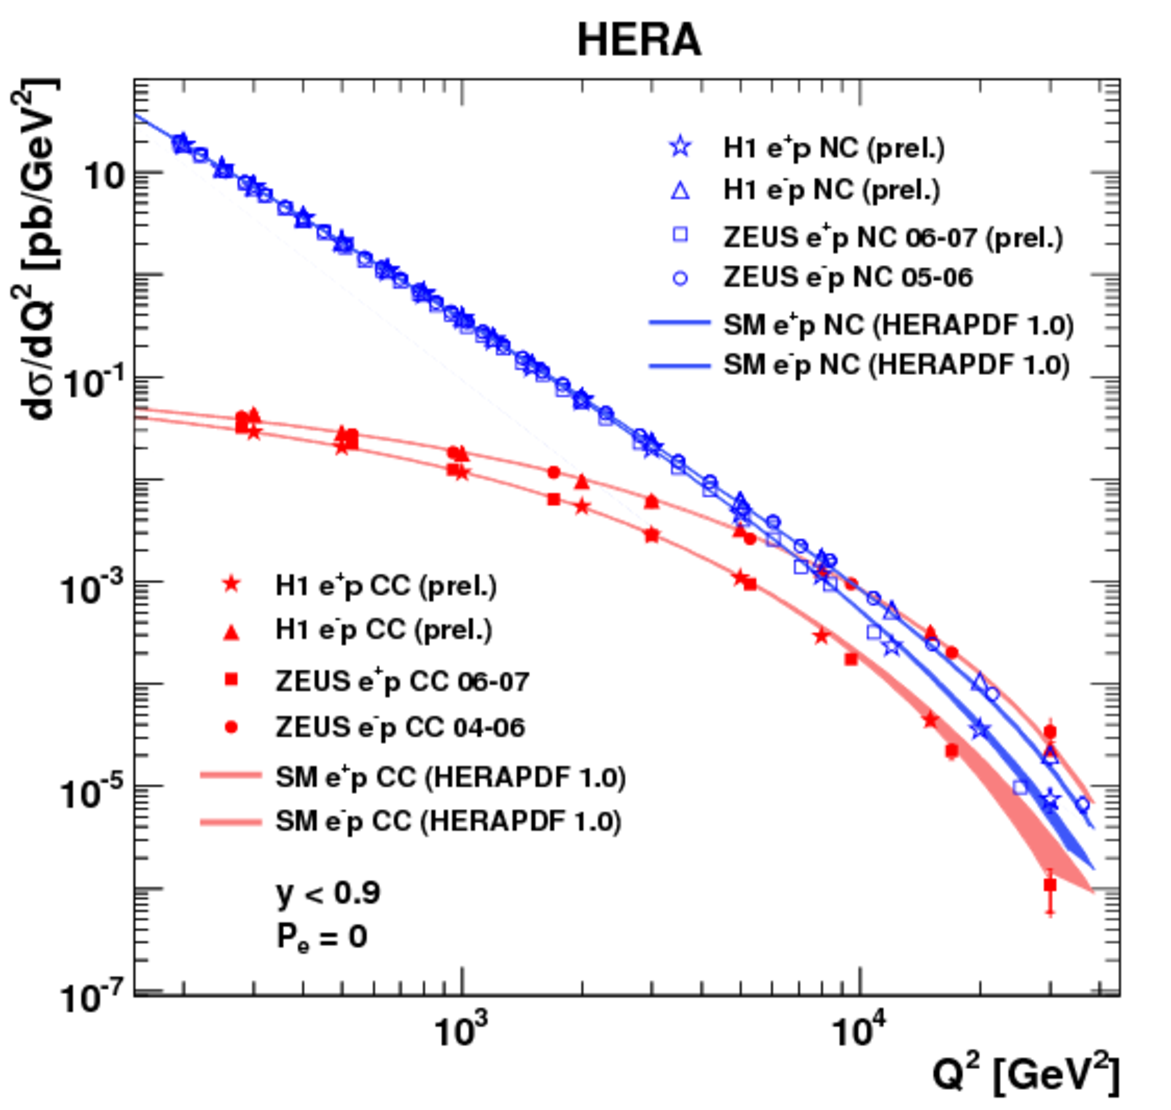
\includegraphics[width=\textwidth]{images/chapter_3/electroweakUnification.pdf}
    \caption[Electroweak unification measurements at HERA]{Neutral current (blue) and charged current (red) differential cross sections as a function of $Q^2$ in $e^\pm p$ collisions, indicating unification at large $Q^2$. \cite{SUSYUnification}}
    \label{fig:ch3_electroweakUnification}
  \end{center}
\end{figure}

\clearpage

\subsection{\texorpdfstring{$\e^+ \e^-$}{EE} colliders}

There have been a multitude of $\e^+ \e^-$ experiments with a centre of mass enery of a few $\gev$ to over $200 \gev$.  There is planning for a linear $\e^+ \e^-$ collider up to $1\tev$.

The charm quark was discovered in 1974 at SLAC (and in a $p \, \textrm{Be}$ experiment at BNL) via the detection of the decay of the bound state, the $J/\psi$ meson.  $m_{J/\psi} \simeq 3.1 \gev$.  A dimuon mass spectrum from the CMS experiment is shown in figure \ref{fig:ch3_mumuspectrumCMS}.

\begin{figure}[!htb]
  \begin{center}
    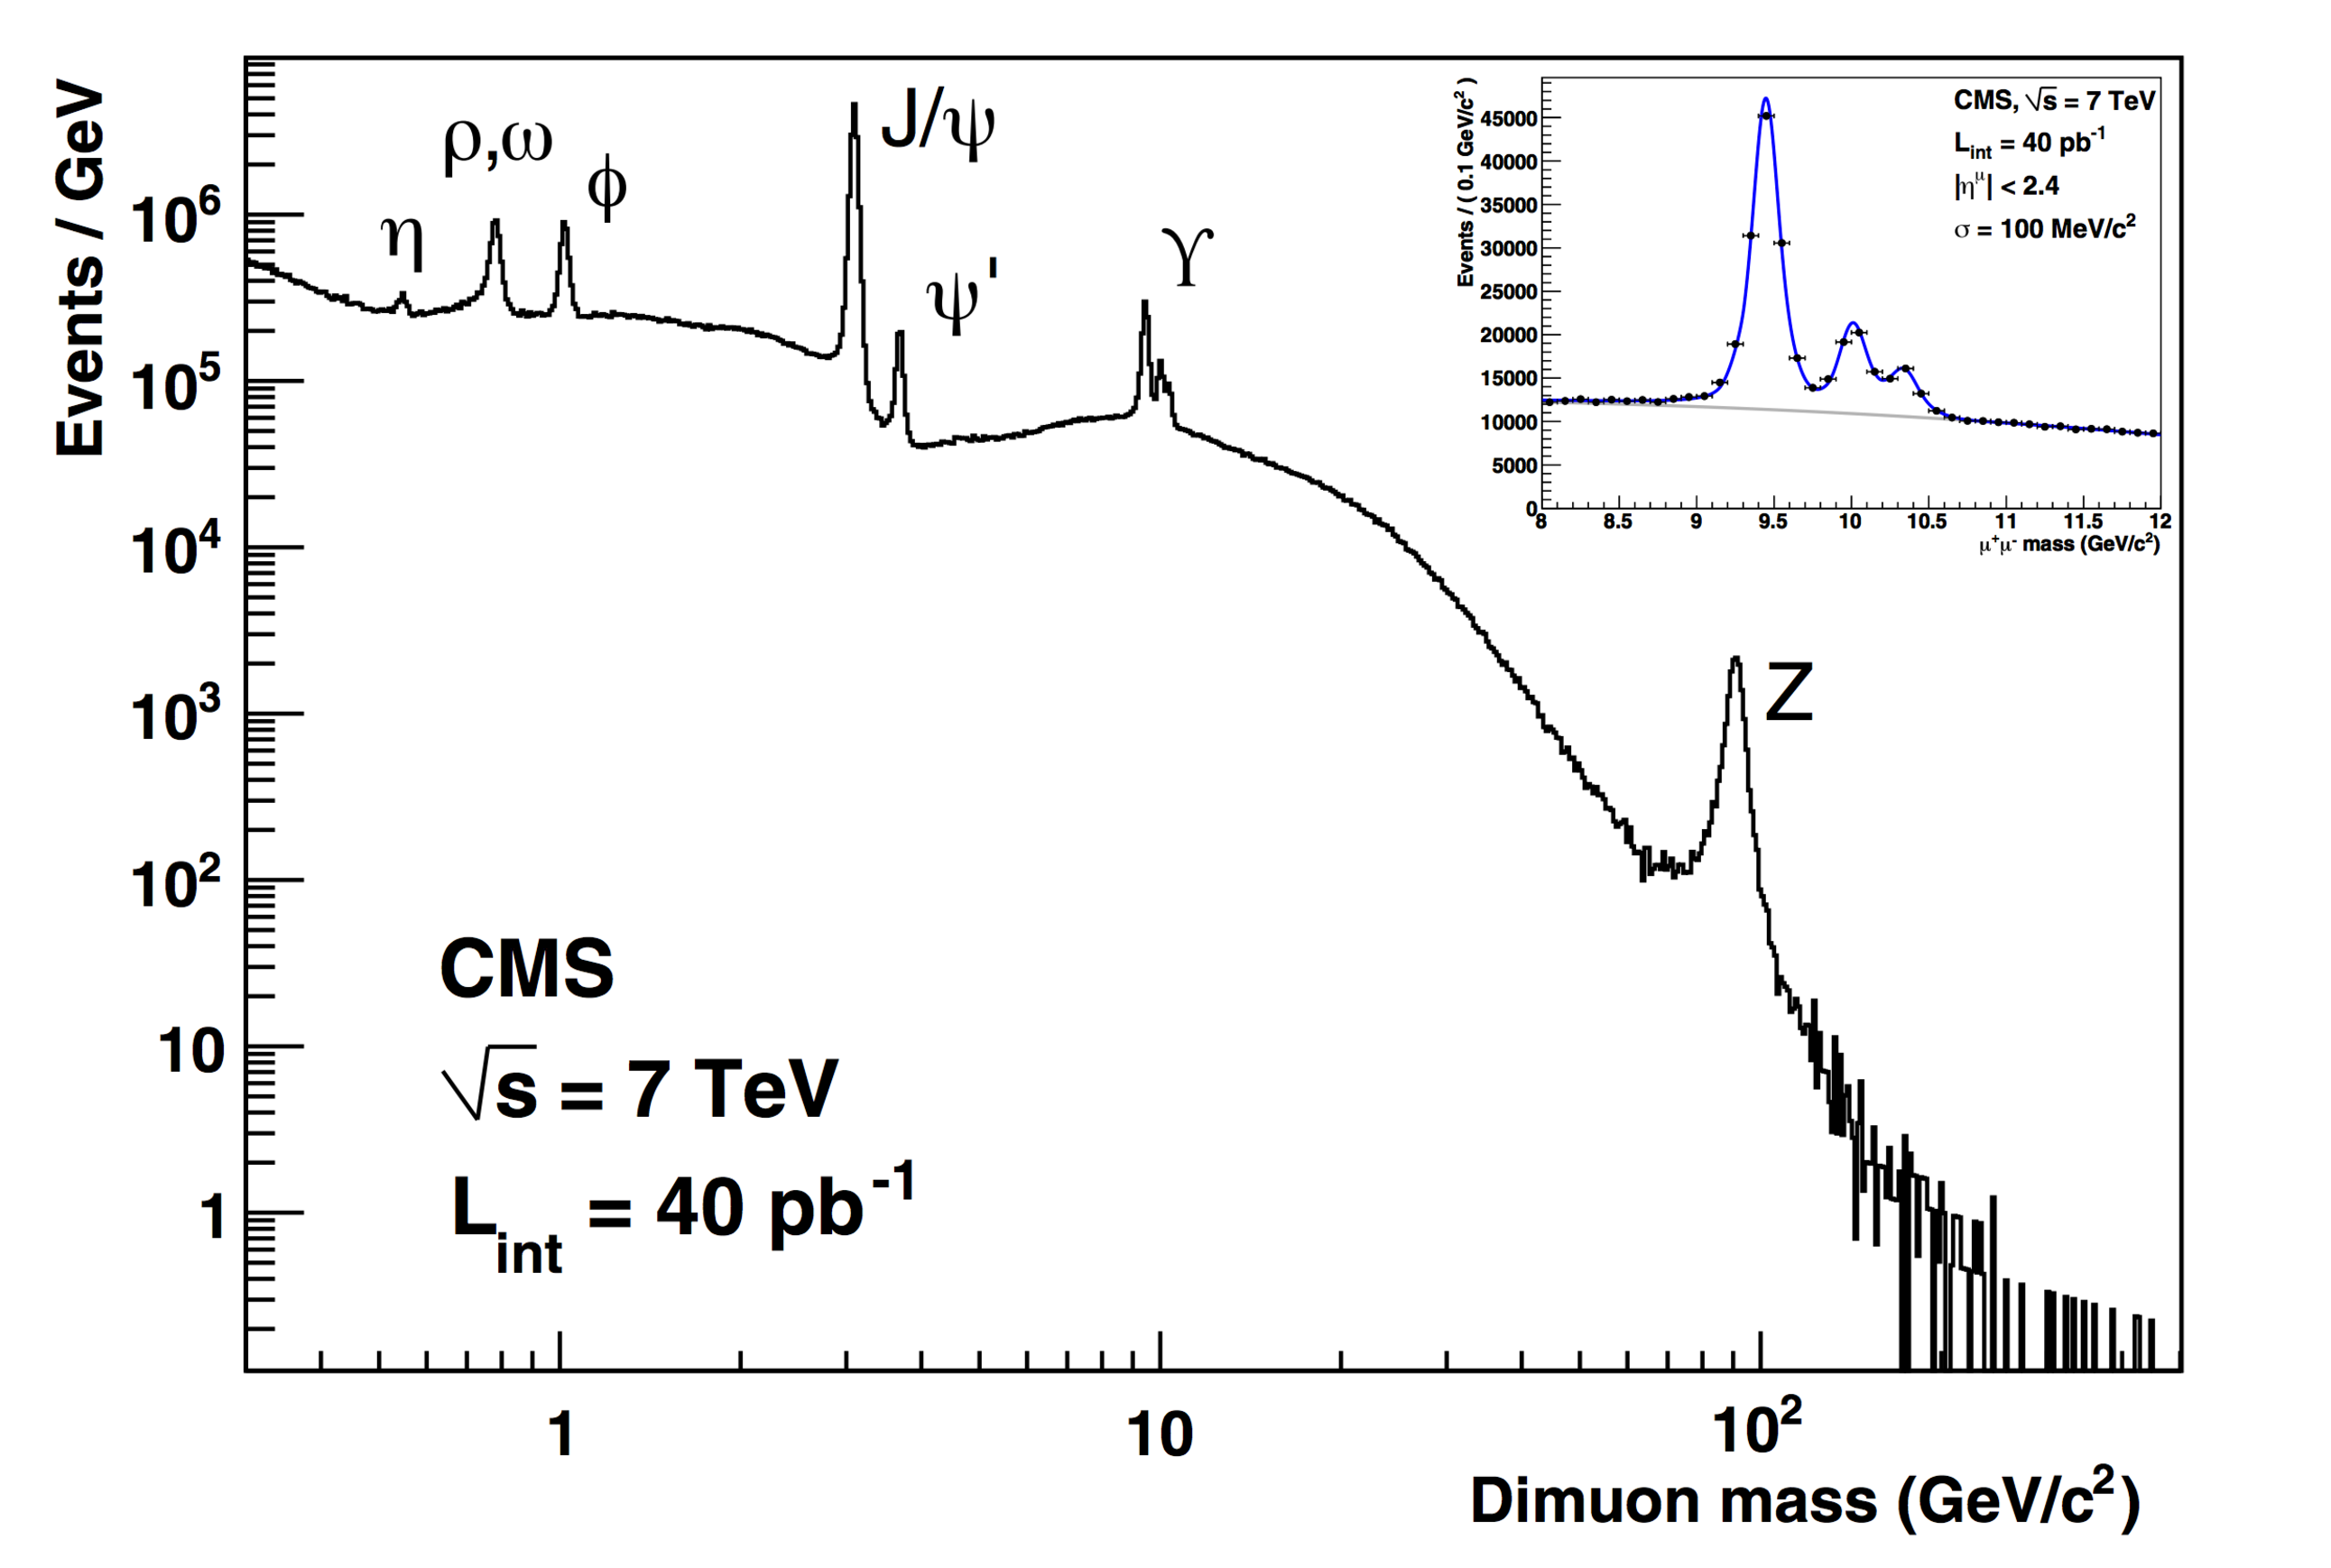
\includegraphics[width=0.9\textwidth]{images/chapter_3/mumuspectrumCMS.pdf}
    \caption[CMS dimuon mass spectrum]{CMS dimuon mass spectrum, over a wide range of masses. \cite{mumuspectrumCMS}}
    \label{fig:ch3_mumuspectrumCMS}
  \end{center}
\end{figure}

In 1979 the gluon was discovered by the experiments at the PETRA collider in DESY at $\sqrt{s} = 35\gev$.  Although $\e^+ \e^-$ is a clean leptonic enviornment, it can provide a powerful probe of QCD eg discovery of the gluon through the oserbvation of $3-$jet events.

Most simply one would expect a srtaightforward process with back to back jets of equal energy.  However, in the detector three jets were seen (one of the quarks radiated a gluon), as indicated in figure \ref{fig:ch3_TwoJetVsThreeJet}.

\begin{figure}[!htb]
  \begin{center}
    \begin{tabular}{c}
      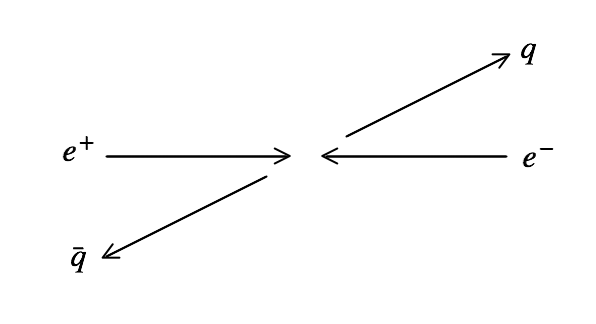
\includegraphics[width=0.6\textwidth]{images/web_feynman/image_14.png} \\
      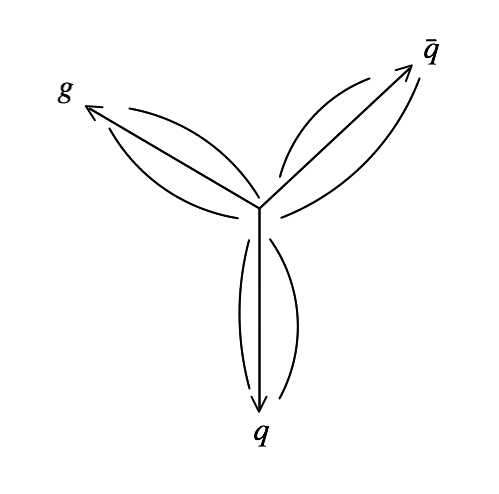
\includegraphics[width=0.6\textwidth]{images/web_feynman/image_15.png}
    \end{tabular}
    \caption[Two and three jet events]{Typical two and three jet events, which were seen at the LEP and HERA experiments.  The Feynman diagrams are shown in the top row and the jet topologies in the transverse plane are shown in the lower row.}
    \label{fig:ch3_TwoJetVsThreeJet}
  \end{center}
\end{figure}

In 1989 the Large Electron-Positron (LEP) collider turned on, embarking on a new era of precision physocs (running at the mass of the $Z^0$ boson.)  Initial LEP running was at the $Z^0$ peak $\simeq 91\gev$, and then moved through $2M_W \simeq 160\gev$ and finally to just over $200 \gev$, looking for the Higgs boson.  There were four multipurpose experiments.  The experiments were most famous for the precision measurements of electroweak parameters such as $M_Z$ and $M_W$.  The measurement of the cross-section as a function of $\sqrt{s}$ was fundamental in measuring $M_Z$ and constraining the number of light neutrinos, as shown in figure \ref{fig:ch3_neutrinos}.

\begin{figure}[!htb]
  \begin{center}
    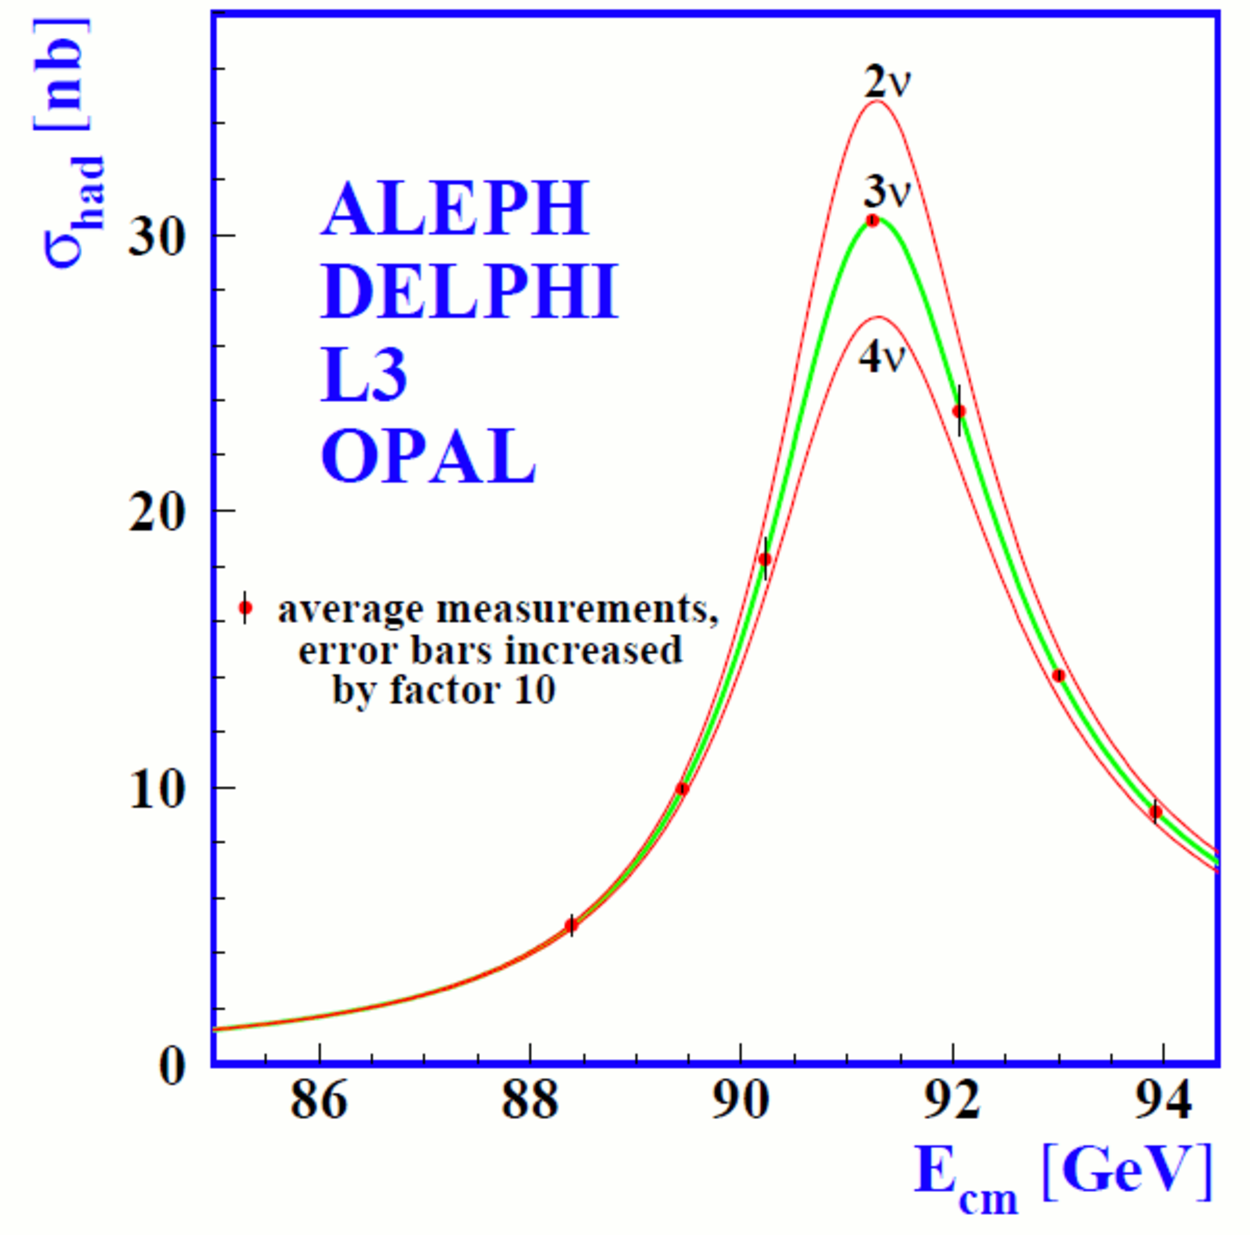
\includegraphics[width=0.8\textwidth]{images/chapter_3/zwidth.pdf}
    \caption[Fit to the number of neutrinos using LEP data]{Fit to the the width of the $Z$ boson to estimate the number of light neutrinos using data from the ALEPH, Delphi, L3 and Opal experiments at LEP. \cite{numberOfNeutrinos}}
    \label{fig:ch3_neutrinos}
  \end{center}
\end{figure}

\begin{eqnarray*}
  M_Z & = 91.1876 & \pm 0.0024 \gev \\
  M_W & = 80.403  & \pm 0.029  \gev
\end{eqnarray*}

In the absence of direct measurements, precise determination of known parameters constrain new physics phenomena eg Higgs boson.  In its final throws LEP also searched for the Higgs boson via Higgstrahlung, where a virtual $Z^0$ results in a real $Z^0$ and Higgs boson.  The process is shown in figure \ref{fig:ch3_EEToHZ}.

\begin{figure}[!htb]
  \begin{center}
    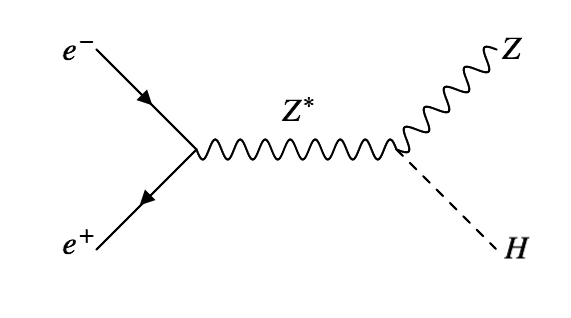
\includegraphics[width=0.8\textwidth]{images/web_feynman/image_16.png}
    \caption[Feynman diagram of $ee\to HZ$]{Feynman diagram showing the process of Higgstrahlung $ee\to HZ$.}
    \label{fig:ch3_EEToHZ}
  \end{center}
\end{figure}

The centre of mass energy was constantly increased as the necessary energy, $E$ had to satisfy $E > M_H + M_Z$, but the Higgs boson was not observed.

Limits of circular $\e^+ \e^-$ machines are being reached due to the rate of energy loss due to synchrotron radiation.

The next planned major collider is the International Linear Collider (ILC).  This would complement the LHC because of the cleanliness of the signal.  This can act as a ``factory'' for eg $t\bar{t}$ production, Higgstrahlung etc.

\subsection{Hadron-hadron colliders}

Due to the hadronic structure and multitude of final states, these colliders are generally more complicated than $\e^+ \e^-$ colliders.  However, they are usually the energy frontier and thereby produce discoveries and measurements of known phenomena over a large kinematic range.

The discovery of the $b$ quark took place in 1977 by obvserving the production and decay of the $\Upsilon$ mesons via $\mu^+ \mu^-$ in $p \quad \textrm{Be}$ collisions at Fermilab.

\begin{figure}[!htb]
  \begin{center}
    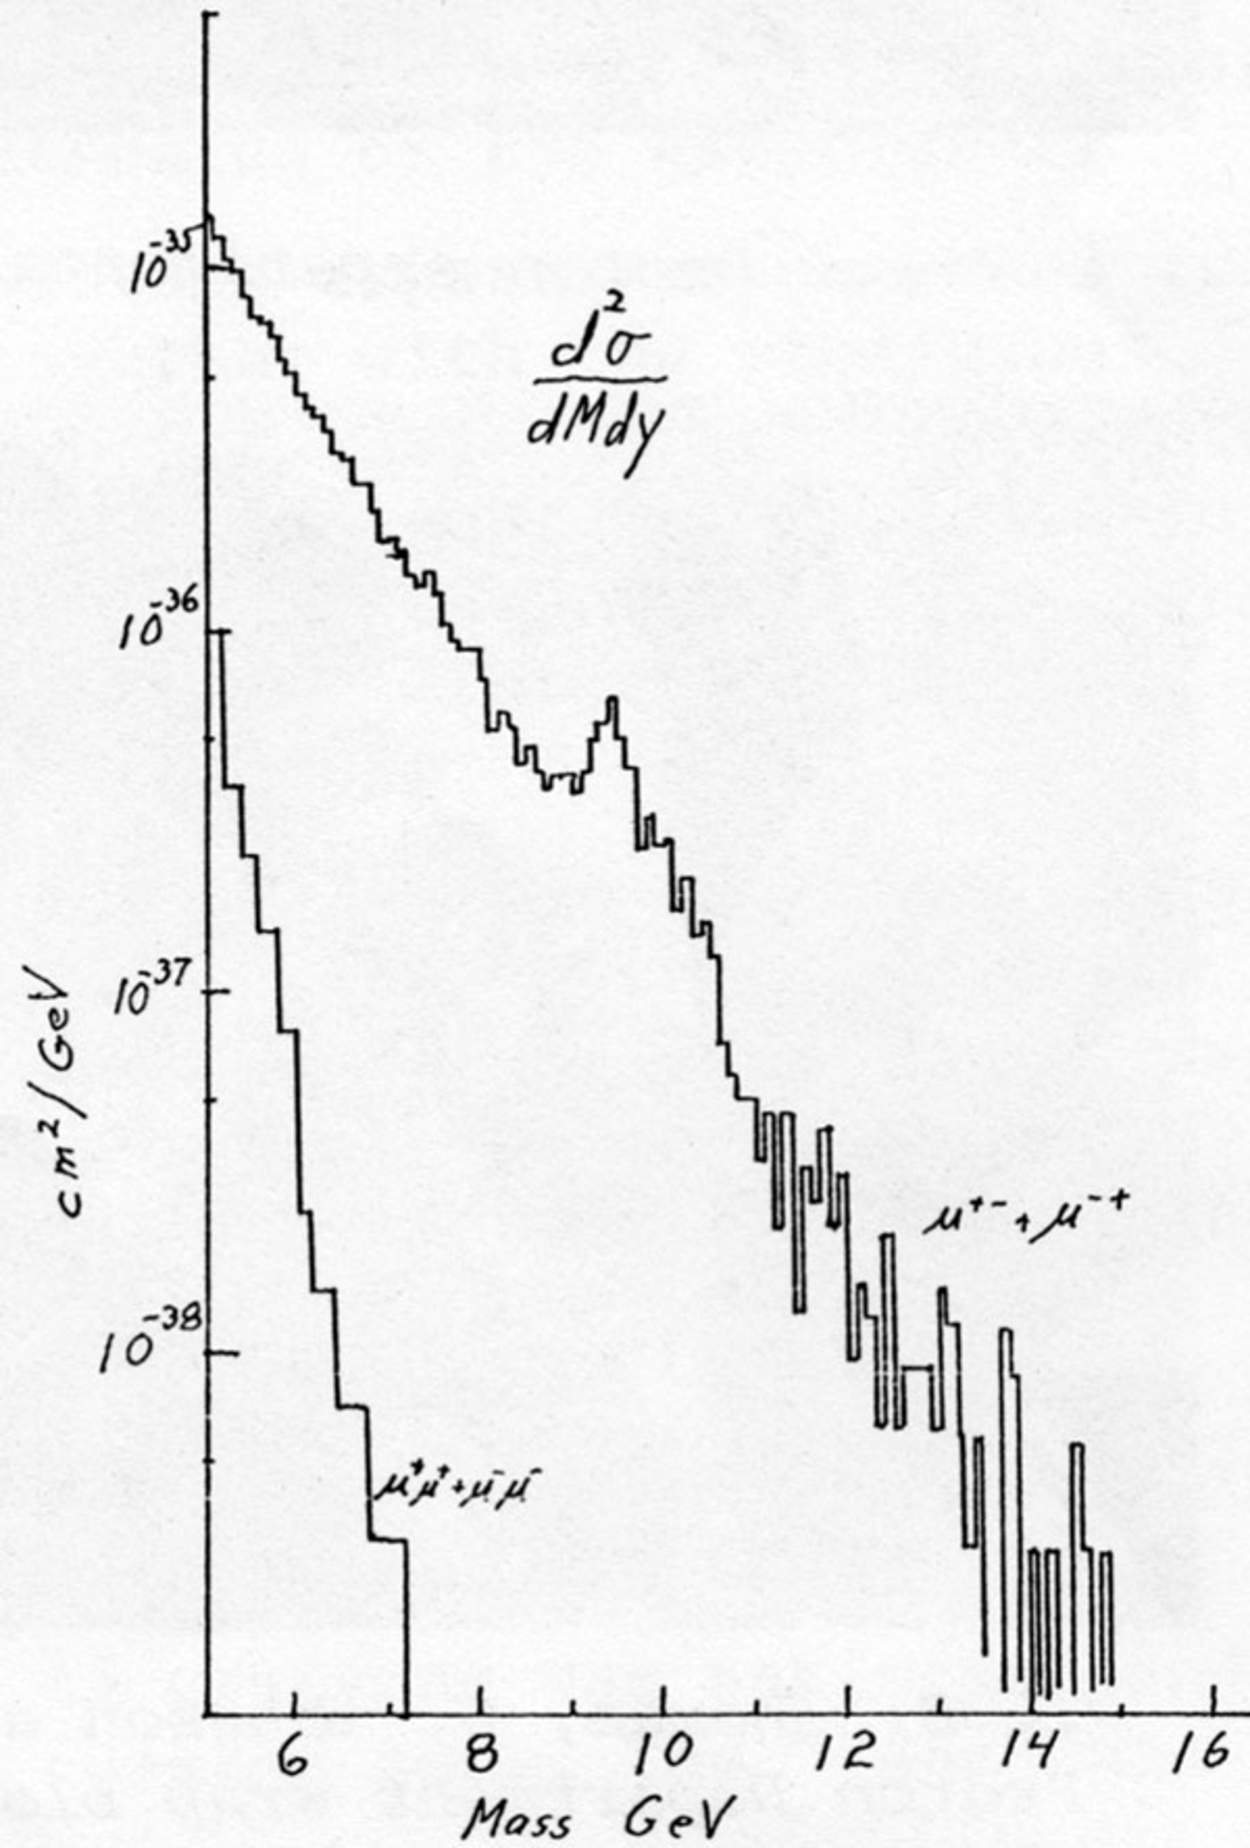
\includegraphics[width=0.75\textwidth]{images/chapter_3/Upsilon.pdf}
    \caption[Discovery of the $\Upsilon(1S)$]{Discovery of the $\Upsilon(1S)$ in the dimuon final state. \cite{Upsilon}}
    \label{fig:ch3_Upsilon}
  \end{center}
\end{figure}

The invariant mass of the $\mu^+ \mu^-$ pair was was observed and a resonance was apparent.

The $W^{\pm}$ and $Z^0$ bosons were discovered in 1984 at the SppS collider at CERN.  Leptonic decays of the $W^{\pm}$ and $Z^0$ were searched for, as they give a lower background relative to hadronic decays ($\sqrt{s} = 540 \gev$).  The top quark was discovered by CDF and D0 at $\sqrt{s} = 1800\gev$ in 1995.

\begin{figure}[!htb]
  \begin{center}
    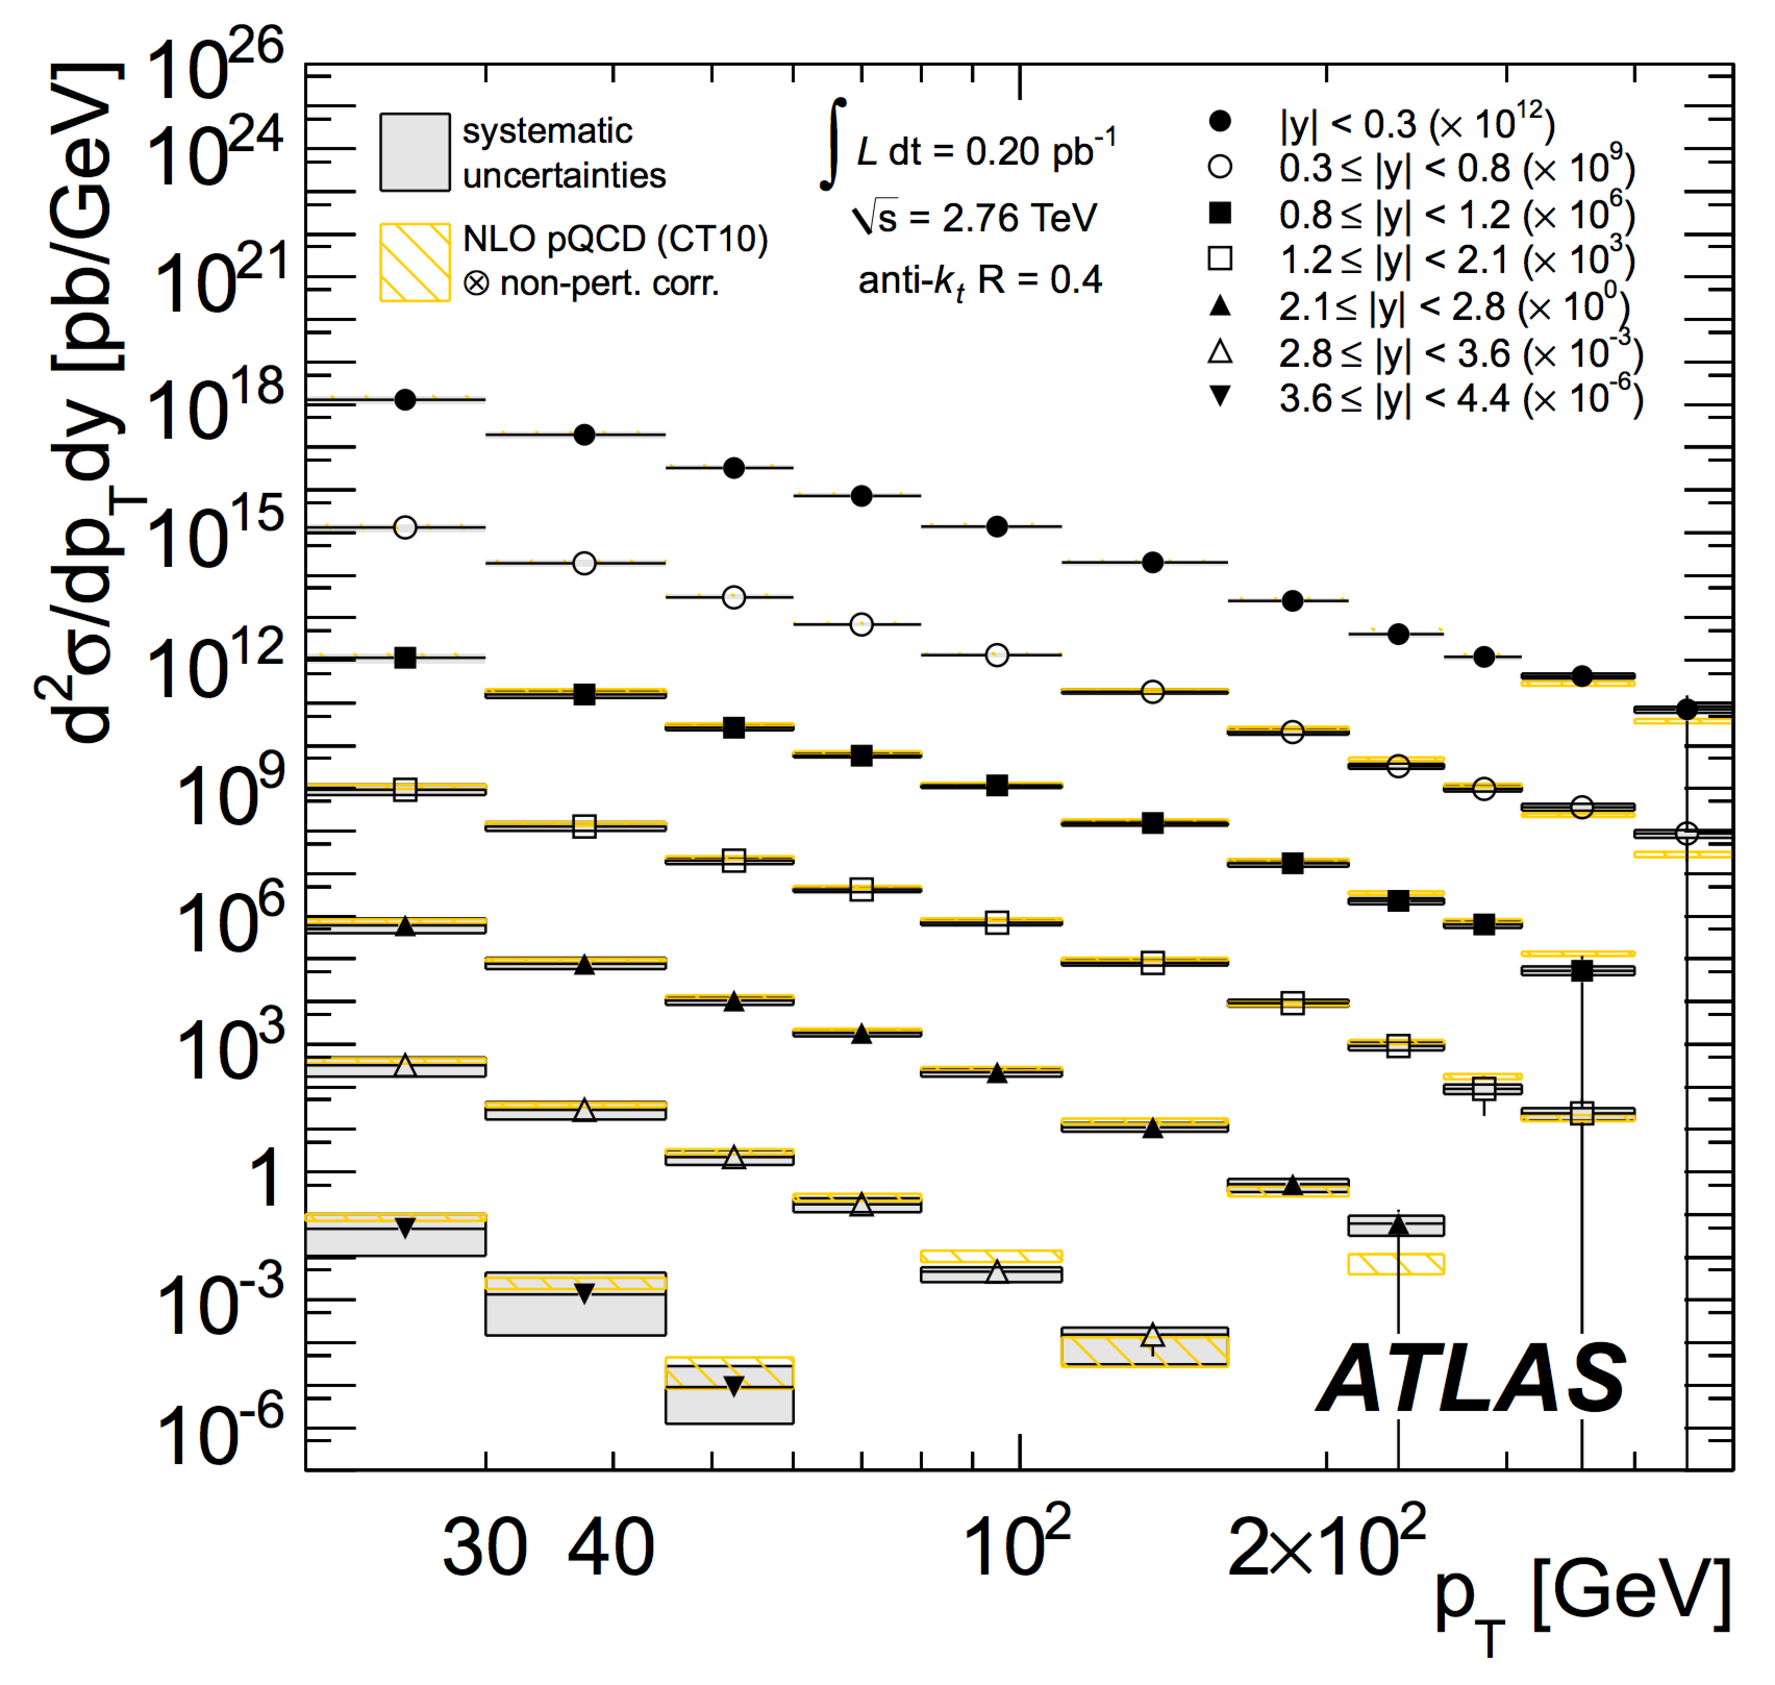
\includegraphics[width=\textwidth]{images/chapter_3/QCD_pt.pdf}
    \caption[Differential cross section of jets]{Differential cross section of jets as function of transverse momentum and pseudorapidity, using data from the ATLAS experiment. \cite{QCD_pt}}
    \label{fig:ch3_QCD_pt}
  \end{center}
\end{figure}

There are high jet energies measures over 24 orders of magnitude in the differential cross-section, as shown in figure \ref{fig:ch3_QCD_pt}.  This allows physicsts to
\begin{itemize}
  \item verify and understand QCD
  \item look for new physics at the highest energies (eg quark substructure)
\end{itemize}